\documentclass[a4paper,10pt]{article}

\usepackage[round]{natbib}
\usepackage{amsmath}
\usepackage{graphicx}

\title{ClonalOrigin in BEAST 2}
\author{Tim Vaughan}

\begin{document}

\maketitle{}

\section{Model}

The model implemented in this package is inspired by the approximation
to the coalescent with gene conversion \citep{Wiuf2000a} used by
\cite{Didelot2010} in their package ClonalOrigin. 

The model is used to find the joint posterior probability density of the
genealogy $G$ of the sample, the coalescent parameters $\theta$, the
substitution model parameters $\mu$ and the recombination rate $\rho$
conditional on the sequence alignment $A$.  This density can be
expanded in the following way
\begin{equation}
f(G,\theta,\mu,\rho|A) \propto P_{\mathrm{F}}(A|G,\mu)f_{\mathrm{CO}}(G|\rho,\delta,\theta)f_{\mathrm{prior}}(\theta,\rho,\mu)
\end{equation}
where $P_{\mathrm{F}}$ is Felsenstein's likelihood for the marginal
trees in $G$ under a substitution model with parameters $\mu$,
$f_{\mathrm{CO}}$ is the density for the gene conversion genealogy
under a modification of the ClonalOrigin model, and
$f_{\mathrm{prior}}$ is the prior density on the continuout
parameters.

We expand the genealogy density in the following way
\begin{equation}
f_{\mathrm{CO}}(G|\rho,\delta,\theta)=f(R|T,M,\theta)P(M|T,\rho,\delta)f_{\mathrm{C}}(T|\theta).
\end{equation}
The density $f_{\mathrm{C}}(T|\theta)$ is simply the density of the
clonal frame $T$ under the standard coalescent model, while the function
$f(R|T,M,\theta)$ is the density of the recombinant edges in the
graph conditional on the number of such edges (via $M$).  These edges
depart from and rejoin $T$ backward in time.  The departure points are
chosen uniformly over the tree, while their points of return are
chosen from conditional coalescent---giving the dependence on
$\theta$.


\begin{table}[t]
\begin{tabular}{|cl|}
  \hline
  Parameter & Definition \\
  \hline
  $A$ & Sequence alignment \\
  $G=\{T,R\}$ & Recombination graph \\
  $T$ & Clonal frame tree \\
  $R$ & Additional edges representing recombinations \\
  $M$ & Set of non-overlapping converted regions of alignment \\
  $\rho$ & Recombination rate (events per unit time) \\
  $\delta$ & Average converted tract length \\
  $\lambda_T$ & Total length of all edges in clonal frame \\
  $L$ & Total length of alignment \\
  $\theta$ & Coalescent rate parameters (e.g. population size model) \\
  $\mu$ & Substitution model parameters \\
  \hline
\end{tabular}
\caption{Description of all parameters used in the model.}
\end{table}


Our model governing the probability of the converted region set $M$
differs from that used by ClonalOrigin. \cite{Didelot2010} allow for
recombination events to affect overlapping regions of the genome.  In
contrast, we forbid the regions from overlapping. Our motivation for
this is twofold: (1) the model for the position of the recombinant edges used
by $f(R|T,M,\theta)$ only makes sense when such overlapping regions
are excluded, and (2) excluding such overlaps leads to simpler and
more efficient code.

Our model for $M$ makes use of the discrete Markov process
\begin{equation}
\begin{bmatrix}
P(s_{k+1}=c|s_1) \\
P(s_{k+1}=r|s_1)
\end{bmatrix}
=
\begin{bmatrix}
1-\frac{\rho' \lambda_T}{2L} & \delta^{-1} \\
\frac{\rho' \lambda_T}{2L} & (1-\delta^{-1})
\end{bmatrix}
\begin{bmatrix}
P(s_{k}=c|s_1) \\
P(s_{k}=r|s_1)
\end{bmatrix},
\end{equation}
where $\lambda_T$ is the total length of all edges in the clonal
frame, $k$ identifies a locus, $s_k\in\{c,r\}$ is the recombination
state of locus $k$ with $c$ indicating sites belonging to the clonal
frame and $r$ representing those which are affected by a
recombination.  Note that the parameter $\rho'$ is related to but does
not \emph{precisely} correspond to the recombination rate $\rho$,
although it provides a good approximation when $\rho'\delta$ is small.

Under this model, the probability for a particular $M$ is written
\begin{align}
  P(M|T,\rho',\delta)&=P(s_1,\ldots,s_L|T,\rho',\delta)\nonumber\\
  &=P(s_1|T,\rho',\delta)\prod_{k=1}^{L-1}P(s_{k+1}|s_k,T,\rho',\delta)
\end{align}
The probability of the state of the first locus can be evaluated by
assuming that the region of loci $[1,L]$ corresponding to our sequence
data is chosen uniformly at random from a longer sequence.  The
probability is then given by the steady state of the chain:
\begin{equation}
P(s_0=c|T,\rho',\delta)=\frac{1}{\frac{\rho'\lambda_T\delta}{2L}+1}=1-P(s_0=r|T,\rho',\delta)
\end{equation}

\begin{figure}[t]
\centering
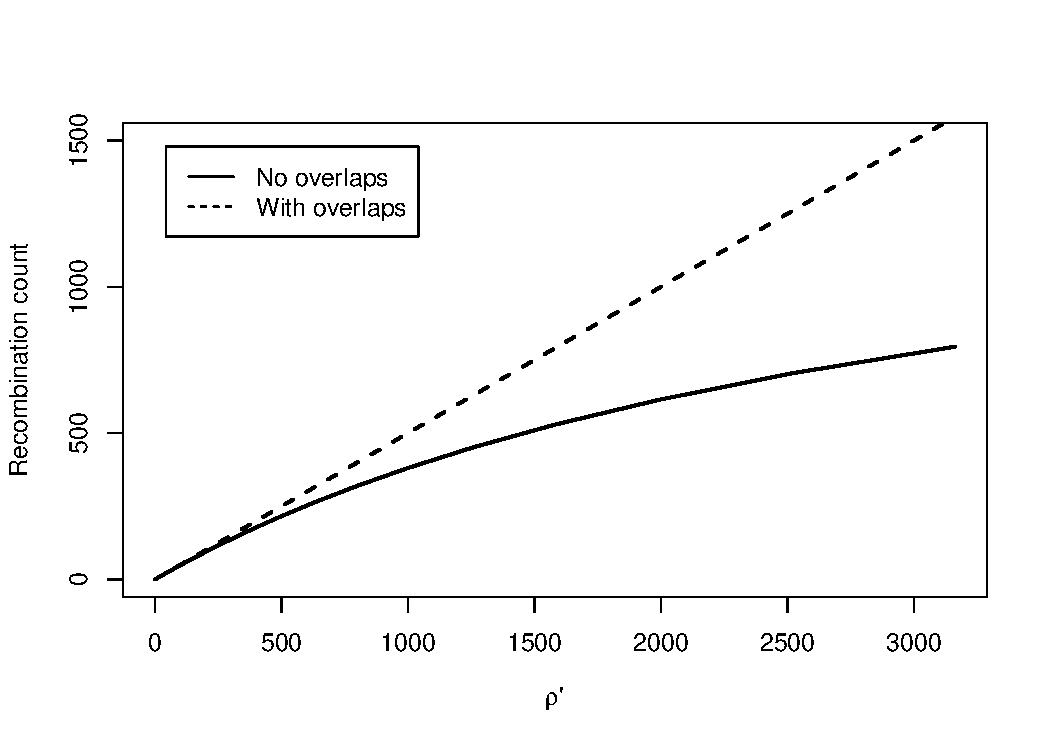
\includegraphics[width=0.8\textwidth]{regionCount.pdf}
\caption{Relationship between parameter $\rho'$ and the number of
recombinations for a $L=1.6\times 10^6$ and $\delta=10^3$ (solid
line).  Relationship when overlapping recombination regions are
allowed is also shown (dashed line).}
\label{fig:recombCount}
\end{figure}

Under this model, the expected number of events along a sequence of
length $L$ is
\begin{align}
N_{\mathrm{rec}}&=\frac{L}{\left(\frac{\rho'\lambda_T}{2L}\right)^{-1}
  + \delta}\nonumber\\
&=\left(\frac{\rho'\lambda_T}{2}\right)\left(\frac{\rho'\lambda_T\delta}{2L}
  + 1\right)^{-1}
\end{align}
This approaches $\rho'\lambda_T/2$ when $\rho'\delta\lambda_T\ll 2L$,
and thus allows us to assume $\rho'\simeq\rho$ in this same limit. In
general, however, the number of recombinations expected under a
particular $\rho'$ is lower than that for the corresponding $\rho$
when overlapping regions are allowed.  This is shown in
figure~\ref{fig:recombCount}.

% We can write $M=\{(x_i,y_i)|i\in[1,q]\}$
% with $q$ being the number of recombinations affecting the sample. The
% elements of each ordered pair $(x_i,y_i)$ define the bounds of the
% region affected by event $i$. Contrary to \cite{Didelot2010}, we
% assume that these regions are non-overlapping and can thus be ordered
% so that $x_1<y_1<\ldots<x_q<y_q$. We apply the constraints $y_1\geq1$
% and $x_q\leq L$, although $x_1$ and $y_q$ are permitted to lie outside
% the sampled sequence.

% Allowing for both a constant recombination rate $\rho$ over the clonal
% frame and a constant average conveted tract length is impossible under
% the non-overlapping assumption.  Thus, we instead write
% \begin{equation}
% %P(M|T,\rho,\delta)= (1-\delta)^{-l}\left(1-\frac{\rho
% %\lambda_T}{2}\right)^{L-l}\left(\frac{\rho\lambda_T}{2\delta}\right)^q
% P(M|T,\rho,\delta) = p
% \end{equation}
% where $\lambda_T$ is the sum of the length of all edges of the clonal
% frame, and $l\equiv\sum_{i=1}^q (y_i-x_i)$ is the total number of
% converted loci. Note that we have made the additional assumption that
% the 




%\bibliography{papers}
%\bibliographystyle{plainnat}

\begin{thebibliography}{2}
\providecommand{\natexlab}[1]{#1}
\providecommand{\url}[1]{\texttt{#1}}
\expandafter\ifx\csname urlstyle\endcsname\relax
  \providecommand{\doi}[1]{doi: #1}\else
  \providecommand{\doi}{doi: \begingroup \urlstyle{rm}\Url}\fi

\bibitem[Didelot et~al.(2010)Didelot, Lawson, Daarling, and
  Falush]{Didelot2010}
Xavier Didelot, Daniel Lawson, Aaron Daarling, and Daniel Falush.
\newblock Inference of homologous recombination in bacteria using whole-genome
  sequences.
\newblock \emph{Genetics}, 186:\penalty0 1435, 2010.

\bibitem[Wiuf and Hein(2000)]{Wiuf2000a}
C.~Wiuf and J.~Hein.
\newblock The coalescent with gene conversion.
\newblock \emph{Genetics}, 155\penalty0 (1):\penalty0 451--462, May 2000.

\end{thebibliography}


\end{document}